\subsection{Relace}
\begin{itemize}
\item \textbf{N-ární relace} nad množinami $A_1, \ldots, A_n$ je \textbf{libovolná podmnožina kartézského} součinu $A_1 \times \ldots \times A_n$ (tyto množiny jsou \textbf{nosičemi} relace).
\item \textbf{Kartézský součin} množin$A$ a $ B $, označovaný $ A \times B $, je množina všech uspořádaných dvojic, kde první prvek z dvojice patří do množiny $ A $ a druhý do množiny$  B $. Příklad: $\{a, b\} \times \{a, b, c\} = \{(a, a), (a, b), (a, c), (b, a), (b, b), (b, c)\}$.
\end{itemize}
\subsubsection{Typy relací}
\begin{itemize}
\item \textbf{homogenní} -- jediný druh nosiče ($A \times A$),
\item \textbf{heterogenní} -- alespoň dva různé druhy nosiče ($A \times B$),
\item \textbf{unární} (n = 1), \textbf{binární} (n = 2), \textbf{ternární} (n = 3), \textbf{n-ární} -- podle arity,
\item \textbf{triviální} -- \textbf{úplná} ($\rho = A_1 \times A_n$), \textbf{prázdná} ($\rho = \emptyset$),
\item \textbf{netriviální} -- $\emptyset \subset \rho \subset A_1 \times \ldots \times A_n$.
\end{itemize}

\subsubsection{Vlastnosti relací}
Binární relace $R \subseteq A \times A$ je:

\begin{itemize}
\item \textbf{Reflexivní} -- $\forall x \in{} A: (x, x) \in{} R $.
\item \textbf{Ireflexivní} -- $\forall x \in{} A: (x, x) \notin{}R $.
\item \textbf{Symetrická} -- $\forall x, y \in{} A: (x, y) \in{}R \Rightarrow (y, x) \in{}R $.
\item \textbf{Asymetrická} -- $\forall x, y \in{} A: (x, y) \in{}R \Rightarrow (y, x) \notin{}R $.
\item \textbf{Antisymetrická} -- $\forall x, y \in{} A: (x, y) \in{}R \land (y, x) \in{}R \Rightarrow x = y$.
\item \textbf{Tranzitivní} -- $\forall x, y, z \in{} A: (x, y) \in{}R \land (y, z) \in{}R \Rightarrow (x,z) \in R$.
\end{itemize}

\subsubsection*{Příklad}
\begin{itemize}
\item Relace ,,$=$'' na $ \mathbb{N} $ je reflexivní, symetrická, antisymetrická a tranzitivní, ale není ireflexivní ani asymetrická.
\item Relace ,,$\leq$'' na $ \mathbb{N} $ je reflexivní, antisymetrická a tranzitivní, ale není ireflexivní, symetrická ani asymetrická.
\item Relace ,,$<$'' na $ \mathbb{N} $ je ireflexivní, asymetrická, antisymetrická a tranzitivní, ale není reflexivní ani symetrická.
\end{itemize}

\subsection{Operace s relacemi}
\begin{itemize}
\item \textbf{Průnik} -- Prvek $ x $ náleží do průniku relací $ R1 \cap R2 $, pokud patří do množiny $ R1 (x \in R1) $ \textbf{a zároveň} do $ R2 (x \in R1)$.
\item \textbf{Sjednocení} -- Prvek $ x $ náleží do sjednocení relací $ R1 \cup R2 $, pokud patří do množiny $ R1 (x \in R1) $ \textbf{nebo} $ R2 (x \in R1)$.
\item \textbf{Doplněk} -- Doplňkem $ R1' $ k relaci $ R1 $ rozumíme \textbf{všechny prvky které nepatří} do $ R1 $.
\item \textbf{Inverze} -- Relace $ R^{-1} \subseteq B \times A $ je inverzní k relaci $ R \subseteq A \times B $, pokud $ xR^{-1}y \Leftrightarrow yRx $.
\item \textbf{Skládání relací} -- Výsledkem je množina dvojic, kde pokud existují dvojice $(a, b)\in R$ a $(b, c)\in S$, pak jejich složení $(a, c) \in R \circ S$.
\end{itemize}

\begin{figure}[H]
	\centering
	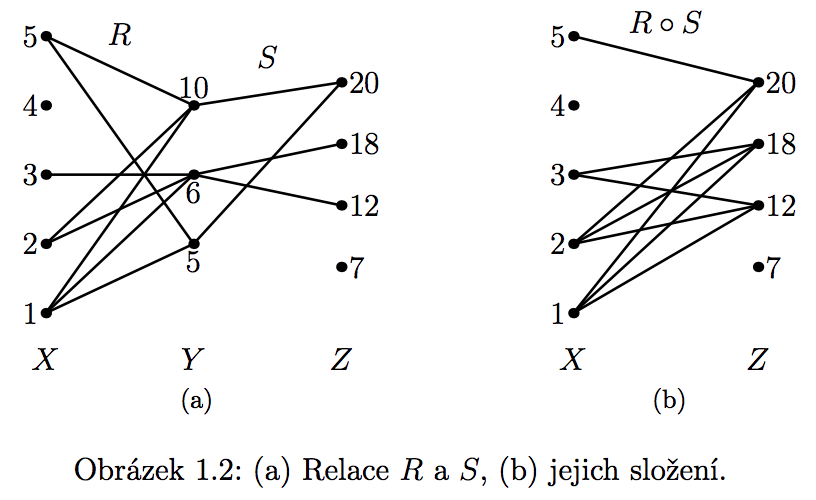
\includegraphics[width=.6\textwidth]{assets/relace_skladani}
\end{figure}

\subsection{Typy binárních relací}
Mezi nejznámější typy binárních relací patří \textbf{ekvivalenece} ($=$) [Re, Sy, Tr], \textbf{uspořádání} ($ <, >, \leq, \geq $) [Re, An, Tr] a \textbf{tolerance} [Re, Sy].

\subsubsection{Ekvivalence [Re, Sy, Tr]}
Relace ekvivalence představuje jakési zjemnění relace rovnosti. Vždy můžeme rozhodnout, že jsou dva prvky množiny stejné, tj. že a = a. Ale někdy se nám hodí zjistit, zda jsou si dva prvky \textbf{pouze podobné}, ne nutně stejné. Neboli zda mají stejnou nějakou zásadní vlastnost. Například dvě knihy můžeme považovat za podobné, pokud mají stejný žánr nebo \textbf{pomocí ekvivalence}: dvě knihy jsou ekvivalentní pokud mají stejný žánr.

\begin{itemize}
\item Binární relace na množině $ X $ je ekvivalentní, pokud je $ R $ na $A$: \textbf{reflexivní}, \textbf{symetrická} a \textbf{tranzitivní}.
\item \textbf{Třída ekvivalence} prvku $ a $ je množina všech prvků ekvivalentních s daným prvkem $ a $.
\item \textbf{Průnik} dvou ekvivalencí je zase ekvivalence.
\item \textbf{Sjednocení} dvou ekvivalencí nemusí znamenat, že výsledek bude ekvivalentní.
\end{itemize}

\subsubsection{Uspořádání [Re, An, Tr]}
\begin{itemize}
\item Binární relace na množině $ X $ je \textbf{neostrým uspořádání}, pokud je $ R $ na $A$: \textbf{reflexivní}, \textbf{antisymetrická} a \textbf{tranzitivní}.
\item Binární relace na množině $ X $ je \textbf{ostrým uspořádání}, pokud je $ R $ na $A$: \textbf{ireflexivní}, \textbf{antisymetrická} a \textbf{tranzitivní}.
\item Uspořádání je \textbf{úplné} pokud neexistují neporovnatelné prvky.
\end{itemize}